\documentclass{sigchi}

% Use this command to override the default ACM copyright statement (e.g. for preprints). 
% Consult the conference website for the camera-ready copyright statement.


%% EXAMPLE BEGIN -- HOW TO OVERRIDE THE DEFAULT COPYRIGHT STRIP -- (July 22, 2013 - Paul Baumann)
% \toappear{Permission to make digital or hard copies of all or part of this work for personal or classroom use is 	granted without fee provided that copies are not made or distributed for profit or commercial advantage and that copies bear this notice and the full citation on the first page. Copyrights for components of this work owned by others than ACM must be honored. Abstracting with credit is permitted. To copy otherwise, or republish, to post on servers or to redistribute to lists, requires prior specific permission and/or a fee. Request permissions from permissions@acm.org. \\
% {\emph{CHI'14}}, April 26--May 1, 2014, Toronto, Canada. \\
% Copyright \copyright~2014 ACM ISBN/14/04...\$15.00. \\
% DOI string from ACM form confirmation}
%% EXAMPLE END -- HOW TO OVERRIDE THE DEFAULT COPYRIGHT STRIP -- (July 22, 2013 - Paul Baumann)


% Arabic page numbers for submission. 
% Remove this line to eliminate page numbers for the camera ready copy
% \pagenumbering{arabic}


% Load basic packages
\usepackage{balance}  % to better equalize the last page
\usepackage{graphics} % for EPS, load graphicx instead
\usepackage{times}    % comment if you want LaTeX's default font
\usepackage{url}      % llt: nicely formatted URLs

% llt: Define a global style for URLs, rather that the default one
\makeatletter
\def\url@leostyle{%
  \@ifundefined{selectfont}{\def\UrlFont{\sf}}{\def\UrlFont{\small\bf\ttfamily}}}
\makeatother
\urlstyle{leo}


% To make various LaTeX processors do the right thing with page size.
\def\pprw{8.5in}
\def\pprh{11in}
\special{papersize=\pprw,\pprh}
\setlength{\paperwidth}{\pprw}
\setlength{\paperheight}{\pprh}
\setlength{\pdfpagewidth}{\pprw}
\setlength{\pdfpageheight}{\pprh}

% Make sure hyperref comes last of your loaded packages, 
% to give it a fighting chance of not being over-written, 
% since its job is to redefine many LaTeX commands.
\usepackage[pdftex]{hyperref}
\hypersetup{
pdftitle={SIGCHI Conference Proceedings Format},
pdfauthor={LaTeX},
pdfkeywords={SIGCHI, proceedings, archival format},
bookmarksnumbered,
pdfstartview={FitH},
colorlinks,
citecolor=black,
filecolor=black,
linkcolor=black,
urlcolor=black,
breaklinks=true,
}

% create a shortcut to typeset table headings
\newcommand\tabhead[1]{\small\textbf{#1}}


% End of preamble. Here it comes the document.
\begin{document}

\title{SIGCHI Conference Proceedings Format}

\numberofauthors{3}
\author{
  \alignauthor  Stephen Gaschignard\\
    \affaddr{Affiliation}\\
    \affaddr{Address}\\
    \email{e-mail address}\\
  \alignauthor Mert Oguz\\
    \affaddr{Affiliation}\\
    \affaddr{Address}\\
    \email{e-mail address}\\    
  \alignauthor Xiang Zhi Tan\\
    \affaddr{Affiliation}\\
    \affaddr{Address}\\
    \email{e-mail address}\\
}

\maketitle

\begin{abstract}
In this paper we describe the formatting requirements for
SIGCHI Conference Proceedings, and this sample file
offers recommendations on writing for the worldwide
SIGCHI readership. Please review this document even if
you have submitted to SIGCHI conferences before, some
format details have changed relative to previous years.
\end{abstract}

\keywords{
	Guides; instructions; author's kit; conference publications;
	keywords should be separated by a semi-colon. \newline
	\textcolor{red}{Optional section to be included in your final version, 
  but strongly encouraged.}
}

\category{H.5.m.}{Information Interfaces and Presentation (e.g. HCI)}{Miscellaneous}

See: \url{http://www.acm.org/about/class/1998/}
for more information and the full list of ACM classifiers
and descriptors. \newline
\textcolor{red}{Optional section to be included in your final version, 
but strongly encouraged. On the submission page only the classifiers’ 
letter-number combination will need to be entered.}

\section{Introduction}

With the enhancement of robotics and artificial intelligence studies, robots have entered our lives in numerous ways. From industrial robots used in factories to everyday electronics like cleaning robots, humans take advantage of the cutting-edge technology that is designed for them. While studies about robotics deal with development and optimization of such technologies, the scope of human robot interaction studies expands through understanding psychological processes which humans come across while interacting with robots. Many notions which are vastly studied for human-human interaction such as trust, harm and perception of mistakes have been extended into human-robot interaction. \cite{freedy2007measurement}. It is clear that robots making mistakes during the interaction, therefore the performance of the robot is one of the most important reasons for trust to diminish. \cite{hancock2011meta}. Whether the other body is a human or robot, people tend to trust if there is consistency in the behavior of the other. Making mistakes on the other hand, is a natural outcome of poor analysis of the enclosing environment, sometimes caused by different deficiencies. Humans have a high try and fail learning capability, besides many creative mistake recovery strategies. With today?s technology, robots are still not as talented as humans in terms of communication with other humans or direct interaction. Therefore, in the upcoming years, we predict that a number of studies will be conducted about the robot-made mistakes. As it is interesting to study why robots make mistake, studying how people perceive those mistakes and how they react in such situations is also crucial for designing successful mistake recovery systems.

Our research question focuses on the human perception of the possible robot mistakes in a restaurant setting. We have decided on this setting since we believe that robot waiters might be conventional in the near future. Restaurants are the places where at least a number of interactions occur between the customer and the waiter. These interactions include physical ones where the waiter brings the menu, dish or the bill. Conventionally, a waiter talks to a customer for getting the order or accepting the payment. These interactions have a psychological effect on the customer. Many customers decide on the amount of tip they wish to give based on the behavior of the waiter. Therefore, we categorized different types of interactions with  We analyzed 3 different types of mistakes with different severity levels. Our research is a within-participant study conducted with 49 participants (26 of them were females) where each participant is a U.S. resident. We hired participants through Amazon Mechanical Turk, paying them for completing our online questionnaire. In order to reach a more random participant population, we used video-based research instead of lab-based live settings. \cite{woods2006comparing} showed that video-based methods have reasonable results for new innovative studies. This approach enabled us to conduct our study with much smaller budget and time spending. Instead, we could focus on the scenarios and the quality of the questionnaire. 6 scenarios (3 types of mistakes: Physical, Psychological, Financial and 2 severity levels: Severe, Non severe) are designed for the study. After watching every video scenario, we asked participants how they attribute responsibility to each of the stakeholders (The robot, programmer of the robot, owner of the restaurant, manager of the restaurant, manufacturer). Then, we asked them what would be their reaction in such situations. We hypothesized that both the type and severity of the mistake will influence participants? distribution of blame. We further predicted that people will blame the robot more for psychological abuse. Our last hypothesis was people will blame the robot for non-severe situations, whereas they will blame other stakeholders for severe situations, if the mistake is a financial exploitation or physical abuse.

\section{Methodology}
\section{Result}
\section{Discussion}
\section{Conclusion}

%
%\begin{figure}[!h]
%\centering
%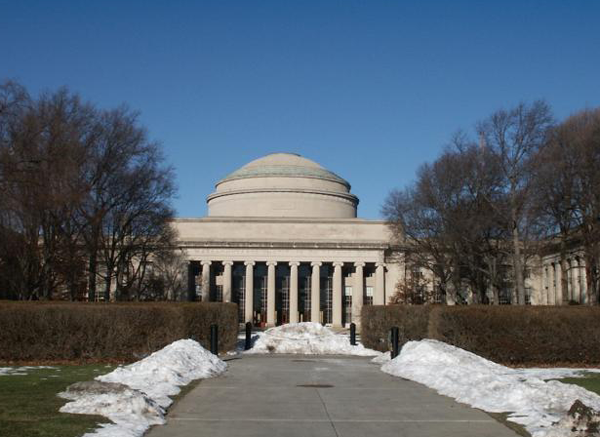
\includegraphics[width=0.9\columnwidth]{Figure1}
%caption{With Caption Below, be sure to have a good resolution image
%  (see item D within the preparation instructions).}
%\label{fig:figure1}
%\end{figure}
%


\section{References format}
References must be the same font size as other body text.
% REFERENCES FORMAT
% References must be the same font size as other body text.
\bibliographystyle{acm-sigchi}
\bibliography{reference}
\end{document}
